%!TEX root = main.tex
 \section{A Sensemaking Model for VQSs\label{sec:sensemaking}}
   %To convey how features in \zvpp address the analytical needs posed by each domain, we organize our PD findings into a sensemaking framework for VQSs. As shown in Figure~\ref{fig:taxonomy}, we develop a taxonomy for organizing VQS capabilities into three sensemaking processes.
 We now revisit Table~\ref{bigfeaturetable} in an effort to contextualize our \rchange{design} findings using Pirolli and Card's sensemaking framework~\cite{Pirolli}. 
 %We demonstrate how features in \zvpp address the analytical needs posed by each domain. We organize the components in Table~\ref{bigfeaturetable} along a taxonomy of three sensemaking processes\cut{, as shown in Figure~\ref{fig:taxonomy}}. %Our VQS sensemaking model is inspired by Pirolli and Card's information foraging framework~\cite{Pirolli}, which distinguishes between information processing tasks that are \textit{top-down} (from theory to data) and \textit{bottom-up} (from data to theory).
 %\change{The sensemaking model was designed for studying how analysts perform ``intelligence analysis'' (bearing semblance to our context of domain experts using VQSs) and related work in visual analytics made use of the sensemaking paradigm to model user behavior~\cite{Battle2016,Yi2008,Srinivasan2019}.}
% Correspondingly, %Analogous to top-down and bottom-up information processing tasks in the sensemaking framework, i
 \rchange{Pirolli and Card's sensemaking model for expert intelligence analysis distinguishes between information processing tasks that are \textit{top-down} (from theory to data) and \textit{bottom-up} (from data to theory). Correspondingly, in the context of VQSs,} analysts can query either directly based on a pattern ``in their head''~\cite{Sedlmair2012} via \emph{top-down pattern specification} or based on the data or visualizations presented to them by the system via \emph{bottom-up data-driven inquiry}. In addition, when analysts do not know what attributes to visualize, \emph{context creation} helps analysts navigate across different collections of visualizations to seek visualization attributes of interest. \cut{A more detailed articulation of the problem space addressable by VQS and how each sensemaking process fits into this space can be found in Appendix~\ref{appdx:problem_space}.}In this section, we first describe \rchange{the objectives of each sensemaking process, then we discuss} how each sensemaking process is comprised of functional components that address the problem and dataset characteristics of each domain. \cut{For reference, the mapping between specific \zvpp features and these components and processes can be found in \rchange{the left two columns of} Table~\ref{bigfeaturetable}.}
 %The sensemaking model was designed for studying how analysts perform ``intelligence analysis'' (of which VQS is a subset of ----- ) and related work in visual analytics have been often applied the sensemaking model for model user behavior in visual analytics~\cite{Battle2016,Yi2008
 %\cut{(the top level in Figure~\ref{fig:taxonomy}). Proceeding to the lower level of the Figure~\ref{fig:taxonomy} taxonomy,}
% We provide usage scenarios to exemplify how each sensemaking process enables essential subtasks towards our participants' scientific goals (further detailed in  Table~\ref{science_task} in Appendix~\ref{apdx:pdartifact}).
 %\npar Table~\ref{science_task} illustrates how each of the subtasks in participant's workflow can be addressed by a sensemaking process.
   %ahen the visualized attributes are unknown to the users
 %, then we outline the design challenge addressed by each of the functional components that supports the sensemaking process
   % In this section, we first describe the space of problems addressable by VQSs.
   % After understanding how each sensemaking process fits into the problem space addressable} by VQSs,
   %  we further explore design objectives of each sensemaking process, grounded in our collaborative design experience.

   % \cut{
   %  \begin{figure*}[ht!]
   %  \centering
   %  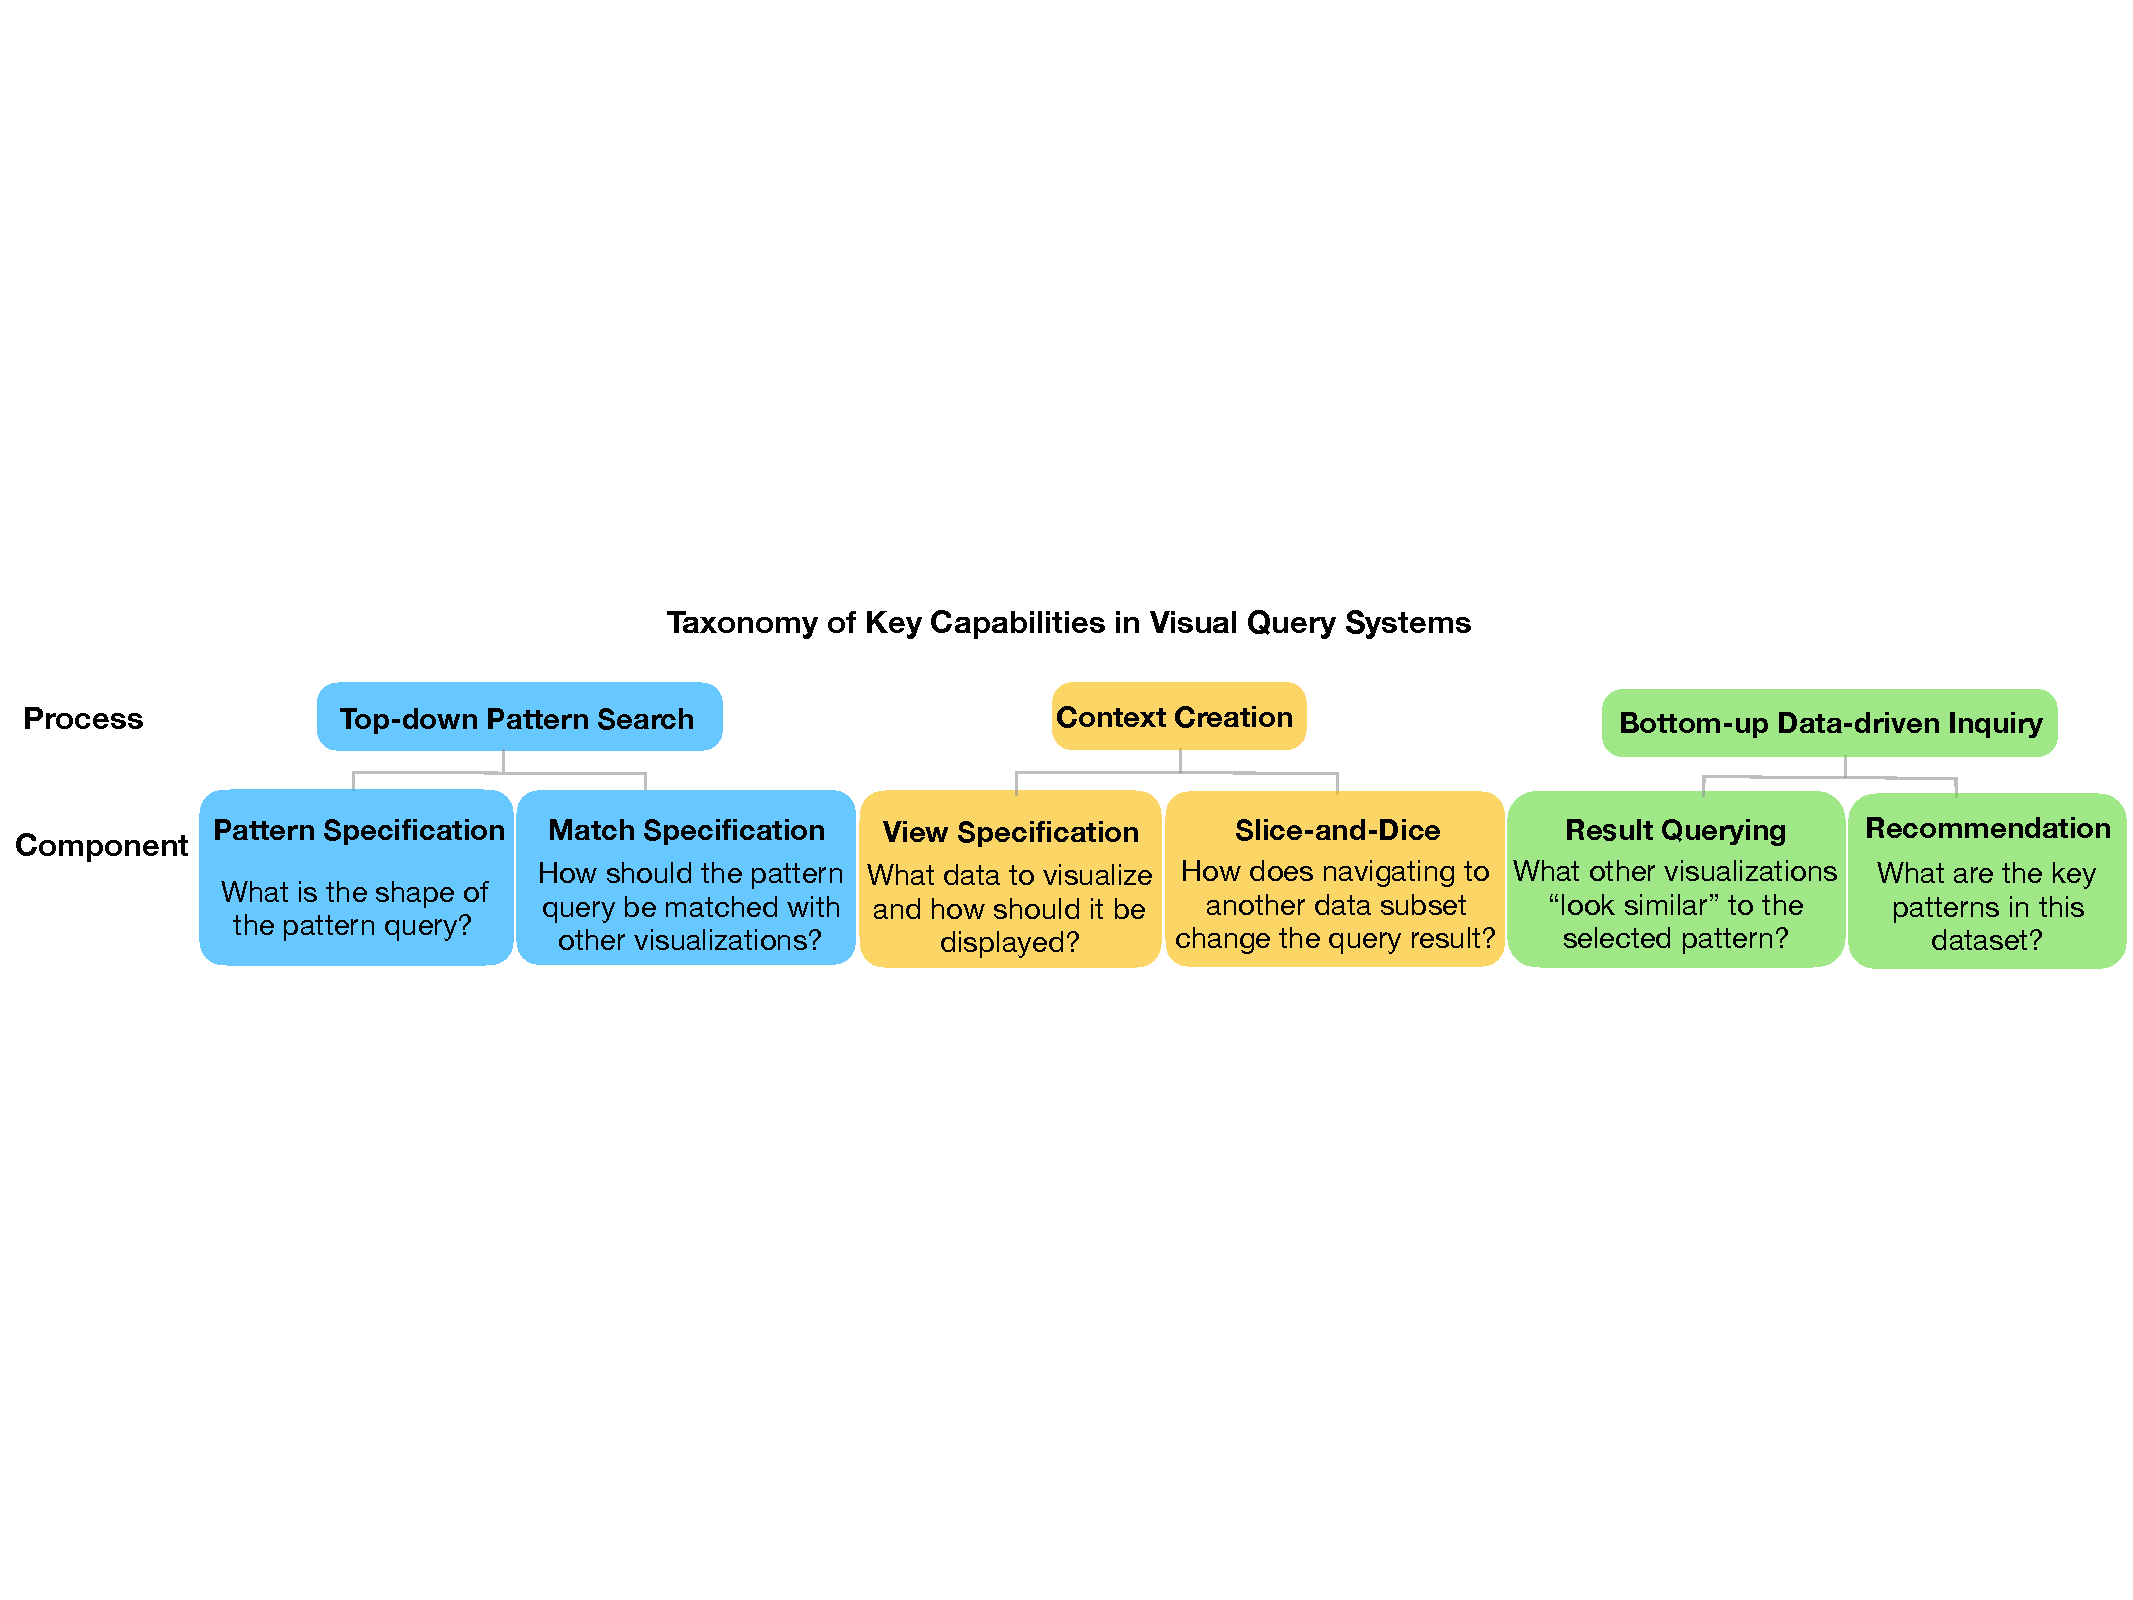
\includegraphics[width=0.9\linewidth]{figures/taxonomy.pdf}
   %  \caption{Taxonomy of key capabilities essential to VQSs. Each of the three sensemaking process is broken down into key functional components in VQSs. Each component addresses a pro-forma question from a system's perspective.} %, which is instantiated as features in \zvpp.}% The bottom-most layer connects the use cases features that have practical or envisioned usage based on the evaluation study.}
   %  \label{fig:taxonomy}
   %  \vspace*{-10pt}
   %  \end{figure*}
   % }
   \subsection{Top-Down Pattern Search}
   Top-down processes are ``\textit{goal-oriented}'' tasks that make use of ``\textit{analysis or re-evaluation of theories [and] hypotheses [to] generate new searches}''~\cite{Pirolli}. Applying this notion to the context of VQSs, the goal of top-down pattern search is to search for data instances that exhibit a specified pattern, based on analyst's intuition about how the desired patterns should look like ``in theory'' (including visualizations from past experience or abstract conceptions based on external knowledge). Based on this preconceived notion of what patterns to search for, the design challenge is to translate the pattern query from the analyst's head to a query executable by the VQS. This requires both components for specifying the pattern (\textit{pattern specification}), as well as controls governing how the pattern-matching is performed (\textit{match specification}).
   %address the \textit{which} question of visual sensemaking: \textit{which data instances exhibit this pattern?}
   %%%%%%%%%%%%%%%%%%%%%%%%Components%%%%%%%%%%%%%%%%%%%%%%%%%%%%
   \boldpara{Pattern Specification} interfaces allow users to submit exact descriptions of a pattern query. This is useful when the dataset contains \emph{large numbers of potentially-relevant pattern instances}.
   Since it is often difficult to sketch precisely, additional shape characteristics of the pattern query (e.g., patterns containing a peak with a known amplitude, or expressible as a functional form) can be used to further winnow the list of undesired matches.%with the VQS returning a list of most similar matches
   \boldpara{Match Specification} addresses the well-known problem in VQSs where pattern queries are imprecise~\cite{correll2016semantics,Holz2009,Eichmann2015} by enabling users to clarify how pattern matching should be performed. Match specification is useful when the dataset is \emph{noisy}. When the pattern query satisfies some additional constraints (e.g., the pattern is \rchange{horizontally} invariant), adjusting these knobs \cut{helps }prune away matches that are false-positives to help analysts discover true desired candidates.
   \boldpara{Usage Scenario:} A1 knows intuitively what a supernovae pattern should look like and its detailed shape characteristics, such as the amplitude of the peak and the level of error tolerance for defining a match. He \rchange{first} performs top-down pattern search by querying for transient patterns through sketching\rchange{, then adjusts} the match criterion by choosing to ignore differences along the temporal dimension and changing the similarity metric for flexible matching.
   \subsection{Bottom-Up Data-Driven Inquiry}%goes from data to theory to
   In Pirolli and Card's sensemaking model, bottom-up processes are ``\textit{data-driven}'' tasks initiated by ``\textit{noticing something of interest in data}''~\cite{Pirolli}. Likewise in VQSs, bottom-up data-driven inquiry is a browsing-oriented sensemaking process that involves tasks that are inspired by system-generated visualizations or results. The design challenge for VQSs to support bottom-up inquiries is to develop the right set of ``stimuli'' through \textit{recommendations} that could provoke further data-driven inquiries, as well as low-effort mechanisms to search via these pattern instances through \textit{result querying}. As we will discuss later, this process is crucial but underexplored in past work on VQSs. %addresses the \textit{what} questions in visual sensemaking: \textit{what are the patterns of interest in the dataset?}
   %%%%%%%%%%%%%%%%%%%%%%%%Components%%%%%%%%%%%%%%%%%%%%%%%%%%%%
   \boldpara{Recommendations} display visualizations that may be of interest to users based on the current data context. In \zvpp, recommendations comprise of representative trends and outliers, which are useful for understanding common and outlying behaviors when a \emph{small number of common patterns} is exhibited in the dataset. %Understanding \emph{characteristic} patterns in dataset can help analysts discover other pattern queries of interest to jumpstart further queries.
   \boldpara{Result querying} enables users to query for patterns similar to a selected data pattern from the ranked list of results or recommendations. Typically, analysts select visualizations with \emph{semantic or visual properties} of interest and make use of result querying to understand characteristic properties of similar instances.
   \boldpara{Usage Scenario:} G2 does not have an upfront knowledge of what to search for. She learns about the characteristic patterns that exist in the dataset through the representative trends, a form of bottom-up inquiry, as a means to jump-start further queries via result querying, as well as understand groups of data instances with shared characteristics.
   \subsection{Context creation}
   While top-down and bottom-up processes operate on a collection of visualizations with fixed X and Y attributes, context creation operates in the regime where the analyst may be investigating the relationships between multiple different attributes or values of interest. Context creation enables analysts to navigate across different visualization collections to learn about patterns in different regions of the data. The design challenge of context creation is to help users visualize and compare how data changes between these different contexts by constructing visualization collections with different visual encodings (\textit{view specification}) or different data subsets (\textit{slice-and-dice}).%to ensure that context is dynamically reflected across other VQS functionalities through
   %develop features that act as a `lens': navigating users to desired data subsets, visualizing and comparing how the data changes between the different lenses, and ensuring that context is dynamically reflected across other VQS functionalities.
   %%%%%%%%%%%%%%%%%%%%%%%%Components%%%%%%%%%%%%%%%%%%%%%%%%%%%%
   \boldpara{View specification} settings alter the encoding for all of the visualizations on the VQS currently being examined. This ability to work with different collections of visualizations is useful when the dataset is \emph{multidimensional} and the axes of interest are \emph{unknown}. Modifying the view specification offers analysts different perspectives on the data to locate visualization collections of interest.
   \boldpara{Slice-and-Dice} empowers users to navigate and compare collections of visualizations constructed from different subsets of the data. Data navigation capabilities are essential when the dataset has \emph{large numbers of ``support attributes''} that may be related to the visualization attributes (e.g., geographical location may influence the time series pattern for housing prices). Analysts can either make use of pre-existing knowledge regarding these support attributes to navigate to a data region that is more likely to contain the desired pattern (e.g., filtering to suburbs to find cheaper housing) or discover unknown patterns and relationships between different data subsets (e.g., housing prices are lower in winter than compared to summer).% by gaining a better understanding of characteristic patterns in particular data region.
   \boldpara{Usage Scenario:} M1 recognizes salient trends in his dataset such as inverse or linear correlations, but does not have fixed attributes that he wants to visualize or a pattern in mind to query with. Given a list of physical properties of potential interest, he performs context creation by switching between different visualized attributes to understand the dataset from alternative perspectives. He can also dynamically create different classes of data (e.g., solvents with low solubility or have high capacity) to examine their aggregate patterns.
   \par The three aforementioned sensemaking processes are akin to the well-studied sensemaking paradigms of search (top-down), browse (bottom-up), and faceted navigation (context creation) on the Web~\cite{Hearst2009,Olston2003}. Due to each of their advantages and limitations given different information seeking tasks, search interfaces have been designed to support all three complementary acts and transition smoothly between them to combine the strength of all three sensemaking processes. 
   \cut{Similarly for VQSs, our design objective is to enable all three sensemaking processes in \zvpp. }Our \cut{Section~\ref{sec:eval_findings} }evaluation study reveals that this integrative approach not only accelerates the process of visualization discovery, but also encourages hypotheses generation and experimentation.